\documentclass{standalone}
\usepackage{tabu}
\usepackage{pgfplots}
\usepackage{pgfplotstable}
\usepackage{graphicx}
\usepackage{textpos}
\usepackage{savesym}
\savesymbol{checkmark}
\usepackage{dingbat}
\usepackage{booktabs}
\usepackage{array}
\usepackage{siunitx}
\sisetup{detect-all}
\usepackage{multirow}
\usepackage{tikz}
\usepackage{calc}
\usetikzlibrary{calc, positioning, quotes}
\pgfplotsset{compat=1.13}
\definecolor{CB-Pl-blue}{HTML}{a6cee3}
\definecolor{CB-Pd-blue}{HTML}{1F78b4}
\definecolor{CB-Pl-green}{HTML}{b2dF8a}
\definecolor{CB-Pd-green}{HTML}{33a02c}
\definecolor{CB-Pl-red}{HTML}{Fb9a99}
\definecolor{CB-Pd-red}{HTML}{e31a1c}
\definecolor{CB-Pl-orange}{HTML}{FdbF6F}
\definecolor{CB-Pd-orange}{HTML}{FF7F00}
\definecolor{CB-Pl-purple}{HTML}{cab2d6}
\definecolor{CB-Pd-purple}{HTML}{6a3d9a}
\definecolor{CB-Pl-brown}{HTML}{FFFF99}
\definecolor{CB-Pd-brown}{HTML}{b15928}

\begin{document}
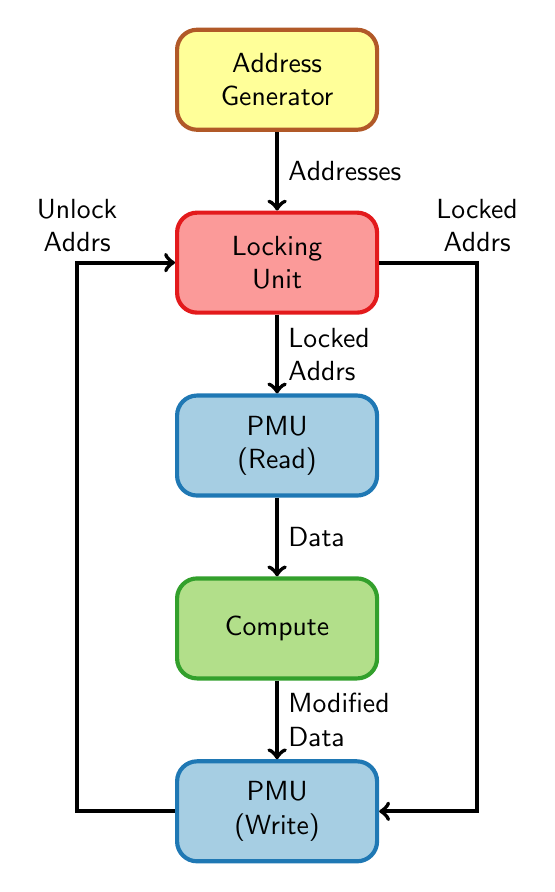
\begin{tikzpicture}
  \sffamily
  \node[fill=CB-Pl-red,draw=CB-Pd-red,rounded corners=0.1in,draw,align=center, minimum width=1in, minimum height=0.5in,line width=1.5pt] (Lock) at (0, 0) {Locking\\Unit};
  \node[fill=CB-Pl-brown,draw=CB-Pd-brown,rounded corners=0.1in,draw,align=center, minimum width=1in, minimum height=0.5in, above=of Lock,line width=1.5pt] (AG) {Address\\Generator};
  \node[fill=CB-Pl-blue,draw=CB-Pd-blue,rounded corners=0.1in,draw,align=center,below=of Lock, minimum width=1in, minimum height=0.5in,line width=1.5pt] (PMUR) {PMU\\(Read)};
  \node[fill=CB-Pl-green,draw=CB-Pd-green,rounded corners=0.1in,draw,align=center,below=of PMUR, minimum width=1in, minimum height=0.5in,line width=1.5pt] (Comp) {Compute};
  \node[fill=CB-Pl-blue,draw=CB-Pd-blue,rounded corners=0.1in,draw,align=center,below=of Comp, minimum width=1in, minimum height=0.5in,line width=1.5pt] (PMUW) {PMU\\(Write)};
  
  \draw[->,line width=1.5pt] (AG) -- node[right,align=left]{Addresses}(Lock) ;
  \draw[->,line width=1.5pt] (PMUR) -- node[right,align=left]{Data}(Comp);
  \draw[->,line width=1.5pt] (Comp) -- node[right,align=left]{Modified\\Data} (PMUW);
  \draw[->,line width=1.5pt] (Lock) -- node[right,align=left]{Locked\\Addrs} (PMUR);
  \draw[->,line width=1.5pt] (Lock) -- ++(1.0in,0) node[above,align=center]{Locked\\Addrs} |- (PMUW);
  \draw[->,line width=1.5pt] (PMUW) -- ++(-1.0in,0) |- node[above,align=center]{Unlock\\Addrs} (Lock);
\end{tikzpicture}
\end{document}
